%%%%%%%%%%%%%%%%%%%%%%%%%%%%%%%%%%%%%%%%%%%%%%%%%%%%%%%%%%%%%%%%%%%%%%%%%%%%%
%%
%% This file provides a template that can be used in concert with the
%% ohio-etd class to generate an electronic thesis or dissertation which
%% meets the formatting requirements at Ohio University.
%%
%% To use the template, copy this file (template.tex) and ohio-etd.cls into
%% the same directory and edit this template as required.  Reference
%% ohio-etd.pdf for additional instructions on using this class.
%%
%%%%%%%%%%%%%%%%%%%%%%%%%%%%%%%%%%%%%%%%%%%%%%%%%%%%%%%%%%%%%%%%%%%%%%%%%%%%%


%% Load the class.  Available options are: numbered, pdftex, cmfont,
%% singlespacetables, draft, 11pt, 12pt, leqno, and fleqn

\documentclass[numbered,pdftex]{ohio-etd}
\usepackage{cite}
\usepackage{notoccite}
\usepackage{amsmath} % Inserting Equations
\usepackage{ragged2e}
\usepackage{verbatim} 
\usepackage{hyperref}
\usepackage{flafter}
\usepackage{color,soul} % Highlighting 

\usepackage{float} % In-text figs
\usepackage{varioref}%  smart page, figure, table, and equation ref
\usepackage{graphicx} % Include graphics
\usepackage{epstopdf} % Figure type .eps to .pdf
\usepackage{wrapfig} % Figures in text
\usepackage{listings}
\usepackage{color} %red, green, blue, yellow, cyan, magenta, black, white
\definecolor{mygreen}{RGB}{28,172,0} % color values Red, Green, Blue
\definecolor{mylilas}{RGB}{170,55,241}
%% Other packages that may be of use.  Delete or comment out (using a
%% percent sign in the first column) if they are not desired.  Reference
%% the corresponding documentation for more information on how to use these
%% packages.

%\usepackage[square,sort&compress,numbers]{natbib} % Provides formatting for
                                                  % citations
\usepackage{textcomp} % Provides math symbols that can be used in text mode
\usepackage{amssymb}  % Provides additional AMS math symbols.  Note that
                      % amsmath is loaded as part of the ohio-etd class
\usepackage{bm}       % Provides bold-faced math symbols
\usepackage{booktabs} % Provides improved table formatting
\usepackage{dcolumn}  % Provides table columns aligned at decimal points
\usepackage{multirow} % Provides table elements spanning multiple rows
\usepackage{graphicx} % Standard package to incorporate graphics
\usepackage[printonlyused]{acronym} % Provides a method for incorporating
                                    % acronyms and building an acronym list

\graphicspath{{figures/}} % Allows graphics files to be stored in a
                          % separate directory
\usepackage{fancyref}
\usepackage{}

%% Required front matter definitions

\degree    {MS}              % MS, MA, MCTP, or PhD
\graduation{December}{2017}    % May, August, or December 

\title     {TITLE}
\author    {Garrett S.}{Clem} 

\advisor   {Jay P. Wilhelm}{Assistant Professor of Mechanical Engineering}
\dean      {Dennis Irwin}{Dean, Russ College of Engineering and Technology }
\program   {Mechanical Engineering}            % e.g. Electrical Engineering
\department{Department of Mechanical Engineering} % e.g. School of Electrical Engineering 
                                    %      and Computer Science
\college   {Russ College of Engineering and Technology}   % e.g. Russ College of Engineering and
                                     %      Technology
\abstract  {ABSTRACT}


%% Optional front matter definitions.  Delete or comment out if not needed

% \coadvisor {Coadvisor's Full Name}{Coadvisor's Full Title}

\dedication{}

\acknowledgments{}
%% If you prefer to provide "acknowledgements" instead (note the added "e"
%% between the "g" and the "m") then add the "e" in the macro name so that
%% it reads "\acknowledgements".}

%% Additional "lists" can be added to the end of the front matter using the
%% \addlistof macro.  For example:
\addlistof{Symbols}{\begin{tabbing}
  XXXX \= \kill% this line sets tab stop
  \\
  $a$ \> Previous or Initial Axial Induction Factor (-) \\


  
 
 
 \end{tabbing}}
%% Note that the command "\input{symbols}" can be used if the symbol list is
%% contained in a separate file called "symbols.tex"}

\addlistof{Acronyms}{

\begin{tabular}{lll}
AoA & Angle of Attack & \\

\end{tabular}}


%% Use "\input{acronyms}" if the acronym list is in a separate file called
%% "acronyms.tex".  Note that the formatting generated by the acronym package
%% can be forced into singlespaced text by inserting "\setlength\itemsep{0pt}
%% \setlength\parskip{0pt}" into the "acronym" environment.} 

%% For documents created by government employees as part of their
%% employment.  The wording of the disclaimer can be specified using an
%% option.  See the documentation for more information.

% \govtdisclaimer    

% \notables  % Prevent a list of tables from being created
% \nofigures % Prevent a list of figures from being created

\begin{document}

\makefrontmatter    % Creates all of the front matter pages.

% for matlab code entrys
\lstset{language=Matlab,%
    %basicstyle=\color{red},
    breaklines=true,%
    morekeywords={matlab2tikz},
    keywordstyle=\color{blue},%
    morekeywords=[2]{1}, keywordstyle=[2]{\color{black}},
    identifierstyle=\color{black},%
    stringstyle=\color{mylilas},
    commentstyle=\color{mygreen},%
    showstringspaces=false,%without this there will be a symbol in the places where there is a space
%     numbers=left,%
%     numberstyle={\tiny \color{black}},% size of the numbers
%     numbersep=6pt, % this defines how far the numbers are from the text
    emph=[1]{for,end,break},emphstyle=[1]\color{red}, %some words to emphasise
    %emph=[2]{word1,word2}, emphstyle=[2]{style},    
}

%% Body of the text follows, using \chapter, \section, \subsection,
%% \subsubsection, \paragraph, and \subparagraph to generate the
%% section headings.  For convenience, it may be useful to break the
%% full document into separate files, perhaps divided by chapters.  In
%% that case, the files would be loaded here using "\input{filename}"


\chapter{Introduction}
\section{Motivation and Problem Statement}

%%UAVs commercially available, ease of use, inexpensive, open source community, wells supported
%- Unmanned Aerial Vehicles (UAVs) are a powerful robotics tool for military and civilian communities alike
%- Advances in lightweight materials and commercial electronics have increased the payload, range, and overall capability of the crafts
%- Reduced costs have brought the technology to a wide range of communities which have found uses such as surveillance, reconnaissance, aerial photography, delivery, and for defense.
%- As the complexity of tasks increase, the complexity of guidance and control systems increase as well. 
%- Traditionally, guidance and control laws have been separate systems responsible for independent tasks
%- Potential field and vector field methods have blurred the line between the guidance and control systems where they have shared the burden of more complex tasks such as obstacle avoidance and path following
%- Potential field has been effective for obstacle avoidance and goal seeking
%- Fixed wing UAVs have a stall velocity constraint and can not stop at a given point
%- Vector field methods have been effective at providing guidance and control for fixed wing UAVs for converging to and following a path
%- Vector fields can be generated in a number of ways, however a convenient method first introduced in \cite{goncalves_artificial_2009} constructs the field by calculating the integral lines converging to and following the level sets of intersecting surfaces. The intersection of surfaces gauntnesses convergence and provides a scalar multiplication factor for convergence, circulation, and time-varying components of the field. 

Unmanned Aerial Vehicles (UAVs) are powerful robotics tools used by both military and civilian communities alike. Advances in lightweight materials and commercial electronics have increase the range, payload, and reliability of the crafts. Reduced costs have brought the technology to a wide range of communities which have found uses such as surveillance, reconnaissance, and aerial photography to name a few. As the complexity of the tasks increase, the complexity of the guidance and control systems increase as well. Traditionally, guidance and control laws have been regarded as separate systems responsible for independent tasks. Potential field and vector field methods have blurred the line between guidance and control systems, whereas now they have shared the burden of complex tasks such as obstacle avoidance and path following. Potential field has been effective for obstacle avoidance and goal seeking for a singular discrete point, however is not initially intended to be used for tasks such as path following. Vector field methods have been effective at providing guidance and control for fixed wing UAVs for converging to and following a path. Vector fields can be constructed in a number of ways, however a convenient method first introduced in  constructs a field by summing together three components consisting of convergence, circulation, and time varying. The filed is generated by calculating the integral lines converging to and following the level sets of intersecting arbitrary surfaces in n-dimensions. Unlike potential field, vector fields do not take into account the dynamics of a vehicle being provided the guidance which provides no guarantee that the UAV will avoid obstacles. Improving the guidance provided by the vector field for obstacle avoidance may be possible by modifying the circulation term of a vector field as a function of a vehicles state with respect to the obstacle.

\chapter{Introduction}
\section{Motivation and Problem Statement}

%%UAVs commercially available, ease of use, inexpensive, open source community, wells supported
%- Unmanned Aerial Vehicles (UAVs) are a powerful robotics tool for military and civilian communities alike
%- Advances in lightweight materials and commercial electronics have increased the payload, range, and overall capability of the crafts
%- Reduced costs have brought the technology to a wide range of communities which have found uses such as surveillance, reconnaissance, aerial photography, delivery, and for defense.
%- As the complexity of tasks increase, the complexity of guidance and control systems increase as well. 
%- Traditionally, guidance and control laws have been separate systems responsible for independent tasks
%- Potential field and vector field methods have blurred the line between the guidance and control systems where they have shared the burden of more complex tasks such as obstacle avoidance and path following
%- Potential field has been effective for obstacle avoidance and goal seeking
%- Fixed wing UAVs have a stall velocity constraint and can not stop at a given point
%- Vector field methods have been effective at providing guidance and control for fixed wing UAVs for converging to and following a path
%- Vector fields can be generated in a number of ways, however a convenient method first introduced in \cite{goncalves_artificial_2009} constructs the field by calculating the integral lines converging to and following the level sets of intersecting surfaces. The intersection of surfaces gauntnesses convergence and provides a scalar multiplication factor for convergence, circulation, and time-varying components of the field. 

Unmanned Aerial Vehicles (UAVs) are powerful robotics tools used by both military and civilian communities alike. Advances in lightweight materials and commercial electronics have increase the range, payload, and reliability of the crafts. Reduced costs have brought the technology to a wide range of communities which have found uses such as surveillance, reconnaissance, and aerial photography to name a few. As the complexity of the tasks increase, the complexity of the guidance and control systems increase as well. Traditionally, guidance and control laws have been regarded as separate systems responsible for independent tasks. Potential field and vector field methods have blurred the line between guidance and control systems, whereas now they have shared the burden of complex tasks such as obstacle avoidance and path following. Potential field has been effective for obstacle avoidance and goal seeking for a singular discrete point, however is not initially intended to be used for tasks such as path following. Vector field methods have been effective at providing guidance and control for fixed wing UAVs for converging to and following a path. Vector fields can be constructed in a number of ways, however a convenient method first introduced in \cite{goncalves_artificial_2009} constructs a field by summing together three components consisting of convergence, circulation, and time varying. The filed is generated by calculating the integral lines converging to and following the level sets of intersecting arbitrary surfaces in n-dimensions. Unlike potential field, vector fields do not take into account the dynamics of a vehicle being provided the guidance which provides no guarantee that the UAV will avoid obstacles. Improving the guidance provided by the vector field for obstacle avoidance may be possible by modifying the circulation term of a vector field as a function of a vehicles state with respect to the obstacle.

\section{Methods Overview}
The Gonsalves vector field method will be applied to generate attractive and repulsive vector fields for the purposes of converging to and following a path while avoiding obstacles. The circulation term of the vector field can be modified to increase the contribution of circulation around the target. Developing the modified vector field guidance will be done in three distinct phases consisting of function development, function evaluation through simulation, and finally validation through simulating a fixed wing UAV on a non-holonomic ground robot.


\section{Phases}
\subsection{Phase I}
\textbf{Construct time parametrized functions for the circulation term of the vector field dependent on common flight measurements.} Common states measured by a UAV include position, closing velocity and heading. Varying the circulation contribution to the total vector field as a function of the vehicles state will be useful for reducing the risk of the UAVs controls being saturated and entering the region the obstacle is occupying.  


\subsection{Phase II}
\textbf{Simulate and compare the parametrized circulation functions with a non-parametrized vector field guidance for circular obstacles.} The performance of the parametrized circulation functions developed in \textbf{Phase I} will be evaluated for a range of vehicle turn rate constraints and obstacle radii. Distance traveled, control effort exerted, and time taken will be used to compare the performance of each parameterized function of circulation to determine which function is the most effective. 


\subsection{Phase III}
\textbf{Simulate a fixed wing UAV with a ground robot guided by the modified vector field guidance to validate simulation results and demonstrate real time guidance is achievable with parametrized circulation modification}. The parameterized circulation function vector field will be implemented on a mobile robot simulating the constraints of a fixed wing aircraft for the purposes of validating the use of the algorithm for real time robotic guidance and control.

\section{Summary of Objectives}
\begin{itemize}
	\item \textbf{Construct time parametrized functions for the circulation term of the vector field dependent on common flight measurements.}
	\item \textbf{Simulate and compare the parametrized circulation functions with a non-parametrized vector field guidance for circular obstacles.}
	\item \textbf{Simulate a fixed wing UAV with a ground robot guided by the modified vector field guidance to validate simulation results and demonstrate real time guidance is achievable with parametrized circulation modification}
\end{itemize}



\chapter{Literature Review}
\section{Introduction to Literature Review}
The following sections provide a discussion on the literature in regards to the modeling of fixed wing unamnned aerial vehicles and the navigation, guidance, and control systems that govern the behavior of the crafts. First, the fixed wing is introduced and a brief discussion on the modeling techniques commonly used for navigation, guidance, and control design. An overview of the structure of autopilots that execute the models is presented. Then, an overview of navigation, guidance, and control is given along with the cutting edge techniques for guidance. (Revisit this section when a rough draft is complete)


\section{Fixed Wing Unmanned Aerial Vehicle}
\subsection{Introduction to Fixed Wing UAV}
Fixed wing unmanned aerial vehicles (UAVs) have seen an increase in use performing tasks such as surveillance, reconnaissance, environmental surveying, aerial photography, and competitive racing. A large spectrum of fixed wing UAVs are in operation today being used by the military and civilians. Larger UAVs may require long stretches of runway to takeoff, while smaller hand launched UAVs do not. Fixed wing UAVs are ideal for tasks that require endurance, high altitude flight, or a large payload. A brief overview of the complex non-linear models used to describe fixed wing UAVs and the simplifications made in literature is discussed, followed by a discussion on the autopilot systems commonly used to control the crafts.

% The models that represent the state of the fixed wing UAV are complex, high dimension, and non-linear. The non linearity is due to the non-linear forces and moments the craft experiences during flight. (Cl, Cd) 
%
%
%
%
\begin{figure}[h]
	\centering
	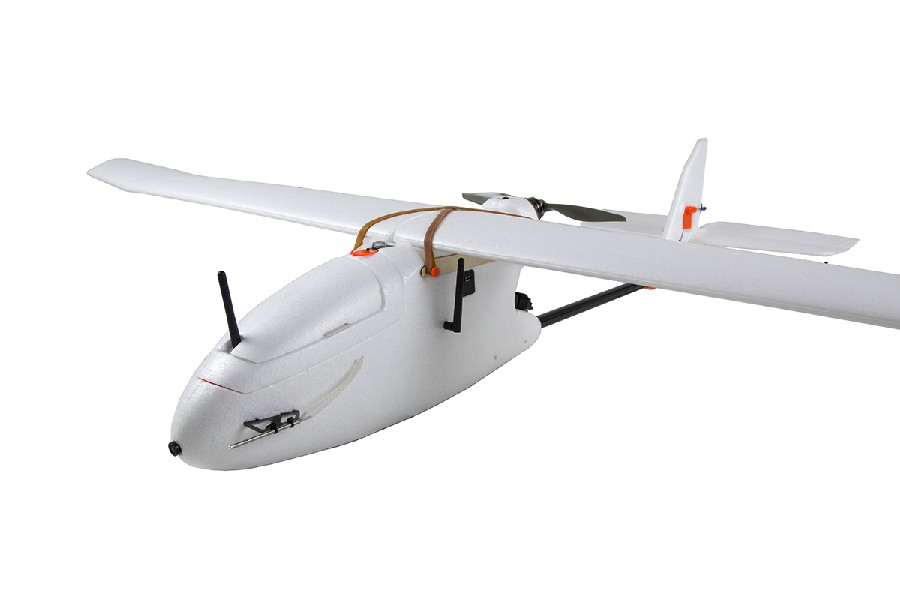
\includegraphics[width=0.7\linewidth]{PaperFigures/fixedwing}
	\caption{3DR Aero}
	\label{fig:fixedwing}
\end{figure}




\subsection{Modeling}
The fixed wing UAV is a 6-DOF system with four degrees of control consisting of pitch, roll, yaw, and thrust. Due to the under-actuation of the craft, several states of the craft are coupled. Lift, pitch, thrust, all of these properties are interconnected and coupled in such a way to produce non-linear high order differential equations which can be difficult to model. Models that represent the position and attitude of the craft as well as the Cartesian velocities and rate of attitude change result in a 12 state variable system of high order non-linear differential equations. 

\begin{figure}[h]
	\centering
	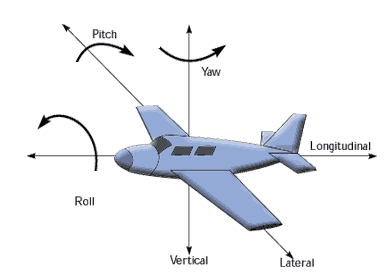
\includegraphics[width=0.7\linewidth]{PaperFigures/pitchrollyaw}
	\caption{Pitch Roll and Yaw}
	\label{fig:pitchrollyaw}
\end{figure}

High order non-linear models can be linearized and simplified to be used in low level control systems to maintain vehicle stability. Beyond the control aspect of UAVs, the high order non-linear models are not always necessary. It is common in literature to simplify the motion of fixed wing UAVs in terms of simple Dubins vehicle kinematic equations \cite{chen_tracking_2009} \cite{liang_tangent_2017} \cite{nelson_cooperative_2005} \cite{griffiths_vector_2006} \cite{jung_unmanned_2016}. When simplified kinematics are used when developing navigation and guidance systems, it is assumed that there already exists a low level control loop that maintains vehicle stability and performs according to the kinematic model in Equations \ref{dubinsx}-\ref{dubinsy}.

\begin{equation}
\label{dubinsx}
\dot{x} = V\cos(\theta)
\end{equation}
\begin{equation}
\label{dubinsy}
\dot{y} = V\sin(\theta)
\end{equation}

The position of the vehicle at any point in 2D Cartesian space is defined as $(x,y)$ and the velocity of the vehicle in each axis is defined as $(\dot{x},\dot{y})$. The heading of the vehicle $\theta$ is most frequently used as the input $\boldsymbol{u} = \theta$. To more closely represent the dynamics of a fixed wing, constraints are given to the velocity $V$ and turning rate $\dot{\theta}$. 

\begin{equation}\label{minVel}
V \geq V_{stall}
\end{equation}
\begin{equation}\label{headingRate}
-\dot{\theta}_{max} \leq \dot{\theta} \geq \dot{\theta}_{max}
\end{equation}

The devices that are assumed to be in control of the UAV when designing guidance and navigation systems are called autopilots or flight controllers, which will be discussed briefly in the next section. 


\subsection{Autopilot}
The autopilot is a software and hardware package that brings navigation, guidance, and control techniques realization. A typical autopilot system is depicted in Figure \ref{fig:pixhawk}, consisting of a hard shell protecting sensors with numerous input and output connectors for power, communication, and servo actuation. The flight controller is responsible for several major tasks including maintaining vehicle stability, turning high level commands into low level control effort, and recording and transmitting data to ground stations. Autopilots accomplish these tasks by implementing several layers of algorithms consisting of navigation, guidance, and control which will be discussed next.

\begin{figure}[h]
	\centering
	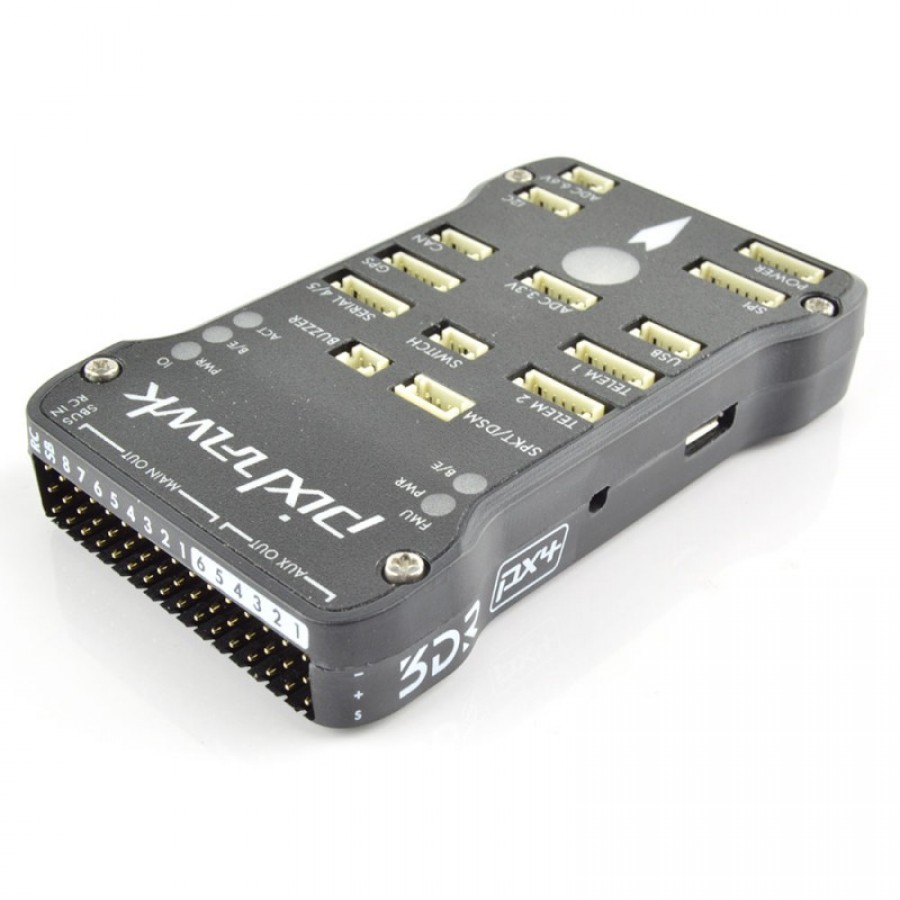
\includegraphics[width=0.7\linewidth]{PaperFigures/pixhawk}
	\caption{Pixhawk Flight Controller}
	\label{fig:pixhawk}
\end{figure}


\section{Navigation, Guidance and Control}
\subsection{Introduction to NGC}
Nearly all of the systems that go into an autopilot system for a fixed wing UAV can be put under the category of Navigation, Guidance, or Control (NGC). Traditionally, NGC could be thought of separate but equally important algorithm layers that aid an autopilot in accomplishing a given task. Navigation is the study of measuring and filtering the state of the vehicle. Guidance produces a commanded state based on high level requests from a path planner or user. Control maintains vehicle stability while attempting to achieve the state commanded by the high level guidance system. Lately, the lines between guidance and control have become less clear as the systems become more integrated with each other, resulting in more complex capabilities. Continuing with the convention in literature, navigation will be discussed as a separate unit while guidance and control will be discussed simultaneously. 

\subsection{Navigation}

Navigation is the study of measuring the position and attitude of the UAV for the purposes of building guidance and providing feedback for the low level control system. Modern flight controllers contain a package of sensors called an Inertial Measurement Unit (IMU) which consists of a 3-axis accelerometer, gyroscope, compass, and barometer. The accelerometer and gyroscope are measured to determine the translational and angular acceleration of the craft. The compass measures the heading, and the barometer measures air pressure which is correlated to altitude. GPS is often used to determine the local position of the UAV. One of the major challenges in navigation is the noise and uncertainty in sensor measurements. Filters are used to fuse information and provide more accurate estimates of the vehicles position and rate of change.


\subsection{Guidance and Control}

%Need more citations on traditional guidance systems for path following to add to the discussion
Guidance and control have traditionally been separate systems, but as the need for UAVs to perform complex tasks increases, so does the complexity of the control systems. A common high level request provided to a UAV is to follow an arbitrary path which can be done with traditional controls [CITATION]. A control system for following a moving path was developed in \cite{oliveira_moving_2016}, which was successful at reducing the tracking error in simulation and real flight tests. To accomplish path following of a mobile path, the control law becomes complex and less intuitive. 

%Needs a better transition and explaination of the control system presented in oliveira 
%Another argument can be made for the distinction between the methods - PF works well for singular point seeking and VF is path seeking
Instead of relying on complex control laws, there has been much research on methods that combine guidance and control.  Two categories will be discussed consisting of potential field and vector field methods. In literature, the two methods have been seen used interchangeably. In the work presented, potential field is in reference to a gradient potential converging to a local minimum while vector field is in reference to a space of vectors whose integral lines converge and follow a path. It can be argued that vector fields are essentially a potential field, but for organizational purposes, they will be referred to as completely different methods. 

\subsection{Potential Field}
- {Introduction to potential field}

Potential field is a real-time robotic manipulator algorithm that distributes the task of goal seeking and obstacle avoidance among multiple layers of control \cite{khatib_real-time_1986}. The robot's workspace is represented as a gradient potential of attractive and repulsive artificial forces that drive the robot to a desired state. Goals are represented as an attractive force while obstacles provide a repulsive force. The potential field is constructed by modeling the robots motion in terms of Lagrangian mechanics shown in Equation \ref{LeeMotion}. The Lagrangian is defined as the difference in kinetic energy $T(x,\dot{x})$ and potential energy $U(x)$ in a system. The goal of the system imparts a potential $U_{xd}$ while obstacles impart a repulsive potential $U_o$. 

\begin{equation}\label{LeeMotion}
\frac{d}{dt} \left(\frac{\partial L}{\partial \dot{x}}\right) - \frac{\partial L}{\partial x} = F
\end{equation}

\begin{equation}\label{lagrange}
L(x,\dot{x}) = T(x,\dot{x}) - U(x)
\end{equation}

\begin{equation}\label{potential}
U_{art}(x) = U_{xd} + U_o(x)
\end{equation}

Potential field has been shown to be successful at driving a robot from an initial state to a goal state while avoiding obstacles by taking the path of least action formed by the gradient. One of the weaknesses of potential field identified early on is the methods susceptibility to local minima, preventing the robot from reaching the desired global minima, or goal state \cite{koren_potential_1991}. Local minima can be avoided in the potential field method if navigation functions are used \cite{goerzen_survey_2010}.\\

Potential field is useful for point-to-point guidance and control which is often the task of UAVs traveling to waypoints, however it is often desired for a UAV to converge to and follow a path. 

%%%%%%%%%% Additional points and clarification needed here before moving on
%
% Address navigation functions
% Re-read Goerzens review article and understand the scope of PF to a better degree
% Improve the transition to vector field
%		- Potential fields have proven to be useful for point-to-point navigation, however lack the framework for one of the common applications for fixed wing UAVs, path following
%
%


\subsection{Vector Field}
{Introduction to Vector Field}

Several methods have been developed to generate vector fields that converge to and follow paths. Histogram virtual force field (VFF) breaks the workspace into discrete cells that contain information in regards to the certainty of the presence of an obstacle \cite{borenstein_real-time_1990} \cite{borenstein_vector_1991}. Cells containing an obstacle apply an artificial guidance force away from the cell. Goals apply a global attractive force that drive the robot towards the desired state. The resultant guidance vector for the VFF method is the sum of the contributions of obstacle repulsive cells and the globally attractive goal. Lyapunov and navigation functions have been successfully used to provide guidance for converging to and following a path. Nelson et al. developed a method for generating a vector field that converges to and follows a path for line and circular primitives \cite{nelson_cooperative_2005}. Sinks, dead zones, and singularities were avoided when constructing more complex flight paths from the primitives by only allowing a single field to be active at any time. A vector field construction method for curved paths was presented in \cite{griffiths_vector_2006} by extending Nelson's method. Elliptical paths have been generated by from primitives by applying coordinate transformations to the field \cite{frew_lyapunov_nodate}.




Vector fields have many advantages to traditional guidance. UAVs often encounter disturbances in the form of wind which can be difficult to plan for. In the event a UAV encounters wind disturbances and is pushed off course, the field will drive the vehicle back on course \cite{de_marina_guidance_2017}. In addition to path following, vector field has been used to track a moving target in 3D \cite{miao_orthogonal_2016}. When the location of the target is unknown, loitering about an uncertain target can be achieved by building a circular vector field and applying a linear coordinate transformation to form an elliptical loiter based on the uncertainty in targets position estimate \cite{frew_cooperative_2007}. 


%
% 3D Vector field 
% \cite{meenakshisundaram_vector_2010}
%
%
%

- Following curved paths in a constant wind \cite{griffiths_vector_2006}


%%%%%% Points to make for vector field
%
% - Disturbance rejection (wind)
% - Well suited for unplanned obstacle avoidance
% - Many applications are best described as path following instead of singular point convergence like potential field
% - Standoff tracking of uncertain targets
%
%

Another method for constructing a vector field is by forming integral curves that converge at the intersection of surfaces \cite{goncalves_artificial_2009}. 

- construct an n-dimensional vector field by forming integral curves that converge at the intersection of surfaces
- Field is a result of the sum of 3 terms
- Convergence
- Circulation
- Time varying\\


% Note, modify the field equation to what jay has in his paper
\begin{equation}\label{gonFieldeq}
\boldsymbol{u} = G\nabla_qV+H\wedge_{i=1}\nabla_q\alpha_i - M(\alpha)^{-1}\boldsymbol{a}(\alpha)
\end{equation}

- Define all variables
- u is the resulting 2x1 vector
- Gradient
- $alpha_i$ is a surface function
- Wedge product simplifies to cross product in 2d
- G, H, L scalar weighting quantities 
- The intersection of the surfaces represents a path to converge and follow
- Cylinder and plane example


\begin{figure}[h]
	\centering
	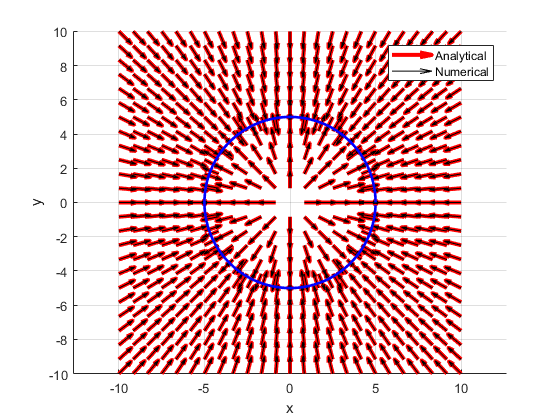
\includegraphics[width=0.7\linewidth]{PaperFigures/convergence}
	\caption{Convergence}
	\label{fig:convergence}
	
\end{figure}

\begin{figure}[h]
	\centering
	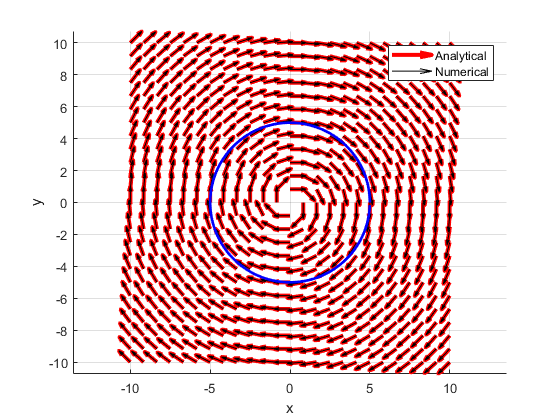
\includegraphics[width=0.7\linewidth]{PaperFigures/circulation}
	\caption{Circulation}
	\label{fig:circulation}
\end{figure}

\begin{figure}[h]
	\centering
	\includegraphics[width=0.7\linewidth]{"PaperFigures/time varying"}
	\caption{Time Varying}
	\label{fig:time-varying}
\end{figure}


\begin{figure}[h]
	\centering
	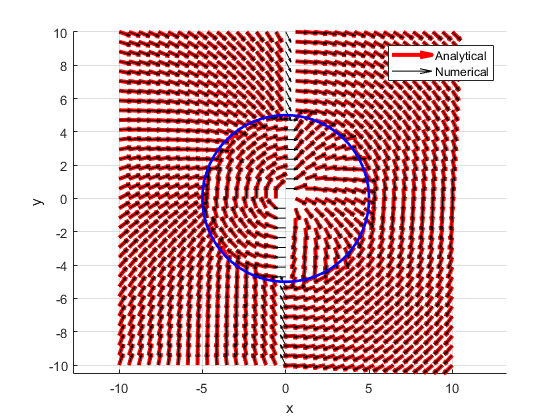
\includegraphics[width=0.7\linewidth]{PaperFigures/total}
	\caption{Total Field}
	\label{fig:total}
\end{figure}

\begin{itemize}
	\item Cooperative Standoff Tracking of Uncertain moving targets (2007, Frew)
	\item VF usefulness extended to loitering about an uncertain target
	\item Lyapunov vector field generation for a circular loiter
	\item Linear transformation applied to stretch the field into an ellipse shape
\end{itemize}





\section{Literature Review Summary}





















\bibliographystyle{aiaa}   
\bibliography{bib}



\end{document}
